\documentclass{book}
\setlength{\parindent}{0cm}
\usepackage[textwidth=17cm,tmargin=3cm,bmargin=2cm]{geometry}

\usepackage[utf8]{inputenc}
\usepackage[french]{babel}
\usepackage{amsmath,amssymb,amsfonts}

\usepackage{graphicx}
\usepackage{psfrag}
\usepackage{caption}
\usepackage{subcaption}
\usepackage{verbatim}

\usepackage{csquotes}
\usepackage{float}

\usepackage{minted}		% Coloration syntaxique
\usepackage[T1]{fontenc}	% Style de ~ incorrect
\usepackage{lmodern}		% Style de ~ incorrect
%\usemintedstyle{upsud}
\newcommand{\inline}[1]{\mintinline[breaklines]{c++}{#1}}

% Meilleures couleurs
\usepackage{xcolor}
\definecolor{red}{RGB}{221,42,43}
\definecolor{green}{RGB}{132,184,24}
\definecolor{blue}{RGB}{0,72,112}
\definecolor{orange}{RGB}{192,128,64}
\definecolor{gray}{RGB}{107,108,110}

\usepackage[onehalfspacing]{setspace}
\setstretch{1.02}

% Solutions encadrées
\usepackage{tikz}
\usepackage[framemethod=tikz]{mdframed}
\newmdenv[
  singleextra={
    \fill[blue] (P) rectangle ([xshift=-15pt]P|-O);
    \node[overlay,anchor=south east,rotate=90,font=\color{white}] at (P) {\sf\textbf{Correction}};
  },
  firstextra={
    \fill[blue] (P) rectangle ([xshift=-15pt]P|-O);
    \node[overlay,anchor=south east,rotate=90,font=\color{white}] at (P) {\sf\textbf{Correction}};
  },
  secondextra={
    \fill[blue] (P) rectangle ([xshift=-15pt]P|-O);
    \node[overlay,anchor=south east,rotate=90,font=\color{white}] at (P) {\sf\textbf{Correction}};
  },
  backgroundcolor=blue!2,
  linecolor=blue,
  skipabove=12pt,
  skipbelow=12pt,
  innertopmargin=0.4em,
  innerbottommargin=0.4em,
  innerrightmargin=2.7em,
  rightmargin=0.7em,
  innerleftmargin=1.7em,
  leftmargin=0.7em,
]{correction}

% Pour cacher/montrer les solutions, décommenter/commenter les 3 lignes ci-dessous
\usepackage{comment}
% \renewenvironment{correction}{}{}
% \excludecomment{correction}

% Fancy chapters
\makeatletter
  \renewcommand{\@chapapp}{TD}
\makeatother

\usepackage{fancyhdr}
\usepackage{fncychap}
  \ChTitleVar{\Huge\bfseries\sffamily\color{blue}}
  \ChNameVar{\raggedleft\fontsize{22}{16}\selectfont\sffamily\color{blue}}
  \ChNumVar{\raggedleft\fontsize{60}{62}\selectfont\sffamily\color{blue}}

% Fancy sections
\usepackage{titlesec}
\titlespacing*{\chapter}{0pt}{-50pt}{40pt}
\titleformat{\section}[block]
  {\Large\bfseries\sffamily\color{blue}}
  {\thesection}
  {1em}
  {}

\newmdenv[nobreak,backgroundcolor=red!20,roundcorner=10pt,linecolor=white]{warning}

\newenvironment{prompt}{\begin{quote}\color{blue!75}\tt\$\,
}{\end{quote}}

\newcommand{\cc}{\mbox{C}}
\newcommand{\cpp}{\mbox{C\vspace{.5em}\protect\raisebox{.2ex}{\footnotesize++~}}}

\def\filename{\texttt}

\usepackage{hyperref}

\begin{document}


\setcounter{chapter}{4}

\chapter{Héritage : polymorphisme et billards}

\begin{center}
  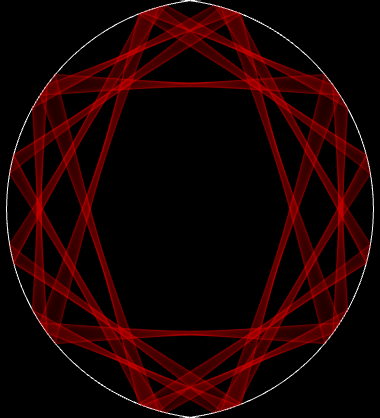
\includegraphics[height=18em]{TD5/exemple-billard.png}
  \hspace{3em}
  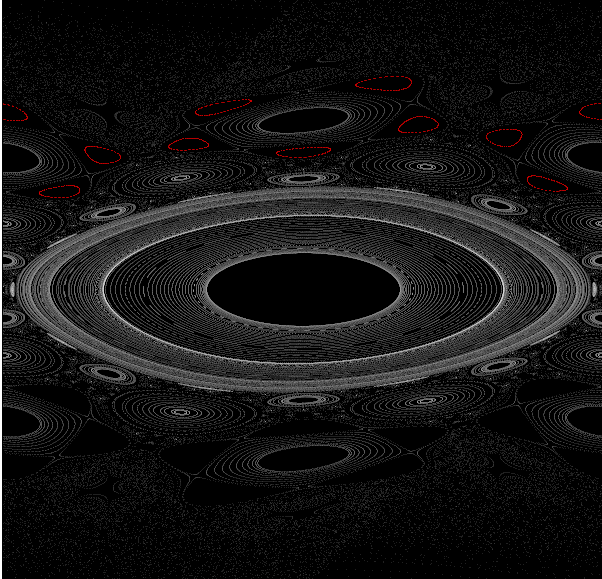
\includegraphics[height=18em]{TD5/exemple-espace-des-phases.png}
\end{center}

Cet ultime TD a pour but d'appliquer la notion d'héritage en créant une famille d'objets représentant des objets physiques : des parois sur lesquelles se réfléchissent des rayons. C'est un cas particulièrement adapté à la programmation orientée objet, et on tirera parti de la notion de \emph{polymorphisme}. On utilisera aussi la bibliothèque graphique SFML pour afficher notre système, ce qui nécessite d'avoir réalisé le TD sur le sujet.

\section{Trajectoires dans un billard}

Pour clore ce cours de \cpp, nous allons développer une simulation de billard au sens des systèmes dynamiques. Wikipedia nous rappelle que

\begin{displayquote}
\textit{Un \href{https://fr.wikipedia.org/wiki/Billard_(mathématiques)}{billard mathématique} est un système dynamique dans lequel une particule alterne des mouvements libres sur une surface et des rebonds sur une paroi, sans perte de vitesse. L'angle de rebond est identique à l'angle d'incidence au moment de choc. Ces systèmes dynamiques sont des idéalisations hamiltoniennes du jeu de billard [...] Les billards mathématiques capturent toute la complexité des systèmes hamiltoniens, de l'intégrabilité au mouvement chaotique [...]}
\end{displayquote}

De façon tout à fait équivalente, la trajectoire d'une particule ponctuelle dans un billard idéal est la même qu'un rayon d'optique géométrique se réflechissant sur des parois-mirroir. Nous allons donc adopter ce second formalisme, en deux dimensions. Une trajectoire sur une scène de plusieurs surfaces/miroirs (ici une surface courbe et une surface rectiligne) ressemblera à :

\begin{center}
  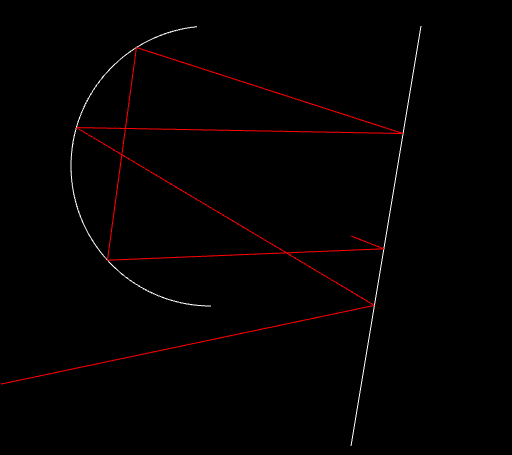
\includegraphics[height=20em]{TD5/reflections-exemples.png}
\end{center}

\subsection{Structure du programme}

Nous allons travailler avec des objets de type \inline{Rayon}, qui ne sont rien d'autre que des demi-droites définies par leur origine et par leur angle par rapport à l'horizontale $\alpha$. Un rayon se propage et rencontre éventuellement une surface.

Nous auront deux types de surfaces réflechissantes :
\begin{itemize}
  \item des segments, représentés par des objets de type \texttt{ObjetReflechissantLigne}
  \item des arcs de cercles, représentés par des objets de type \texttt{ObjetReflechissantArc}
\end{itemize}
Ces deux classes dériveront d'une classe abstraire \texttt{ObjetReflechissant}, exposant une interface commune pour l'interception et le calcul de la réflexion. Une \emph{scène} n'est rien d'autre qu'un ensemble de telles surfaces, et sera représentée par un objet de type \texttt{Scene}, qui stockera et utilisera les \texttt{ObjetReflechissant} de façon polymorphique.\\

Lorsque l'on lance un rayon, que doit on faire ensuite ? Il faut déterminer la première surface (en terme de distance) qui intercepte le rayon. On doit donc tester, pour chaque objet de la scène, si le rayon a été intercepté et à quelle distance. Ceci sera effectué avec une méthode \inline{Réémission interception_réémission (const Rayon& rayon) const}, qui teste si il y a intersection du rayon avec la surface, et renvoie un objet \inline{Réémission}, contenant la distance entre l'origine du rayon et le point d'interception, ainsi que le rayon réfléchi. On sélectionne alors la première surface sur le chemin du rayon, et le rayon ré-émis est alors celui qui a été renvoyé par ladite surface. La logique est résumée sur la figure \ref{fig:intercept-reemit}.a.\\

Pour regrouper la logique commune d'interception et de ré-émission et ne pas avoir à la coder dans chaque classe fille pour chaque géométrie, les calculs d'intersection propres à chaque type de surface seront implémentés par une méthode virtuelle \inline{DonnéesIntersection test_intersection (const Rayon& rayon) const}, qui renvoie si oui ou non le rayon est intercepté, et renvoie éventuellement les paramètres d'intersection suivants (fig.\ \ref{fig:intercept-reemit}.b) :
\begin{itemize}
  \item le point d'intersection 
  \item l'angle d'incidence
  \item l'angle absolu de normale (on choisit la convention de le mesurer par rapport à l'horizontale)
\end{itemize}
qui sont ensuite utilisés par \inline{interception_réémission} pour calculer le rayon réfléchi.

Dans la classe \texttt{ObjetReflechissant}, \inline{test_intersection} sera \emph{abstraite}, c'est-à-dire déclarée virtuelle pure. Son implémentation sera effectuée dans les classes filles \texttt{ObjetReflechissantLigne} et \texttt{ObjetReflechissantArc}. Le point important est que, comme cette méthode est virtuelle, on pourra stocker toutes les surfaces dans un conteneur unique, quelque soit leur type. On est assuré que à l'exécution du programme, la bonne surcharge de \inline{test_intersection} sera appellée en fonction du type de l'objet : c'est le \emph{polymorphisme}.\\

\begin{figure}[H]
  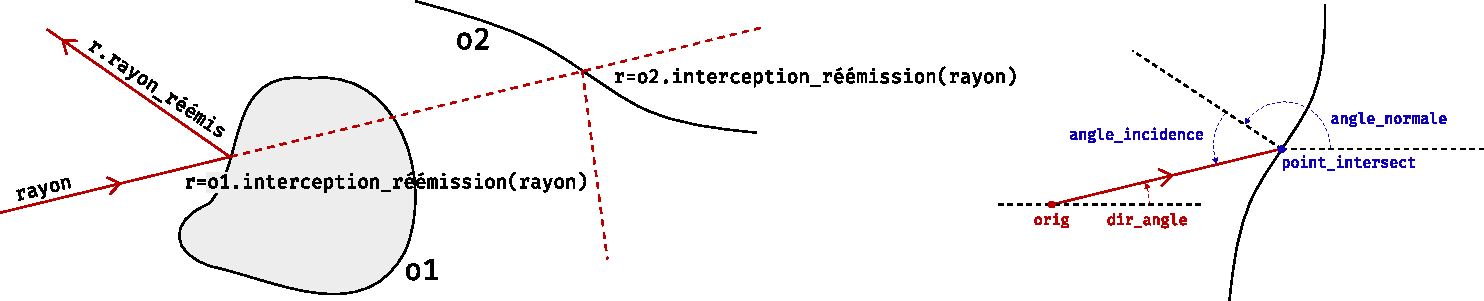
\includegraphics[width=\textwidth]{TD5/intercept-reemit.pdf}
  \caption{À gauche, logique de l'interception d'un rayon avec deux objets \texttt{o1} et \texttt{o2} sur la scène. À droite, paramètres d'intersection en bleu, stockés dans un \inline{ObjetReflechissant::DonnéesIntersection}, et paramètres du rayon (attributs de \inline{Rayon}).}
  \label{fig:intercept-reemit}
\end{figure}

Enfin, \texttt{ObjetReflechissant} déclare une méthode virtuelle \inline{void dessiner (sf::RenderWindow& window) const}, surchargée dans les classes filles, qui dessine la surface dans la fenêtre SFML \inline{window}. Une fois encore, le polymorphisme permettera à la bonne méthode de dessin d'être appellée.\\

Ces trois classes sont schématisées sur le diagramme de classes, fig.\ \ref{fig:diagclasses1}. 

\subsection{Mise en pratique}

Une paire de fichiers \filename{Util.h} / \filename{Util.cpp} est fournie pour gagner du temps. Y sont implémentés les points et vecteurs en 2D (classes \inline{Point2} et \inline{Vec2}), les intervalles angulaires dans $\mathbb{R}/2\pi\mathbb{R}$ (classe \inline{AngleIntervalle}, pratique pour les arcs de cercle), et la "classe" \inline{Rayon}, qui n'est rien d'autre qu'une structure contenant un point et un angle\footnote{On pourrait faire une classe \inline{Rayon} plus raffinée, mais ce TD est déjà assez long comme ça...}. La lecture du code et des commentaires présents dans \filename{Util.h} devraient suffire pour comprendre leur utilisation.\\

On travaillera dans un espace carthésien $[0,1]\times[0,1]$. Pour convertir un \inline{Point2} vivant dans cet espace en une coordonnée de pixel de la fenêtre SFML (\inline{sf::Vector2f}), on pourra utiliser la fonctions \inline{coord_01_vers_fenetre} de \filename{Util.h}. Voici par exemple un code permettant de dessiner une ligne blanche entre deux points \inline{a} et \inline{b} dans une fenêtre SFML \inline{window} :
\begin{minted}[fontsize=\footnotesize,mathescape,xrightmargin=0.5cm,xleftmargin=0.5cm]{c++}
sf::VertexArray line (sf::Lines, 2);
line[0] = sf::Vertex( coord_01_vers_fenetre(a), sf::Color::White );
line[1] = sf::Vertex( coord_01_vers_fenetre(b), sf::Color::White );
window.draw(line);
\end{minted}

Un fichier \filename{Makefile} est fourni, lisez-le. Si la SFML n'est pas dans un répertoire système, ajoutez les options de compilation (\texttt{-I}, \texttt{-L}, \texttt{rpath}...) nécessaires.

\begin{figure}[H]
  \centering
  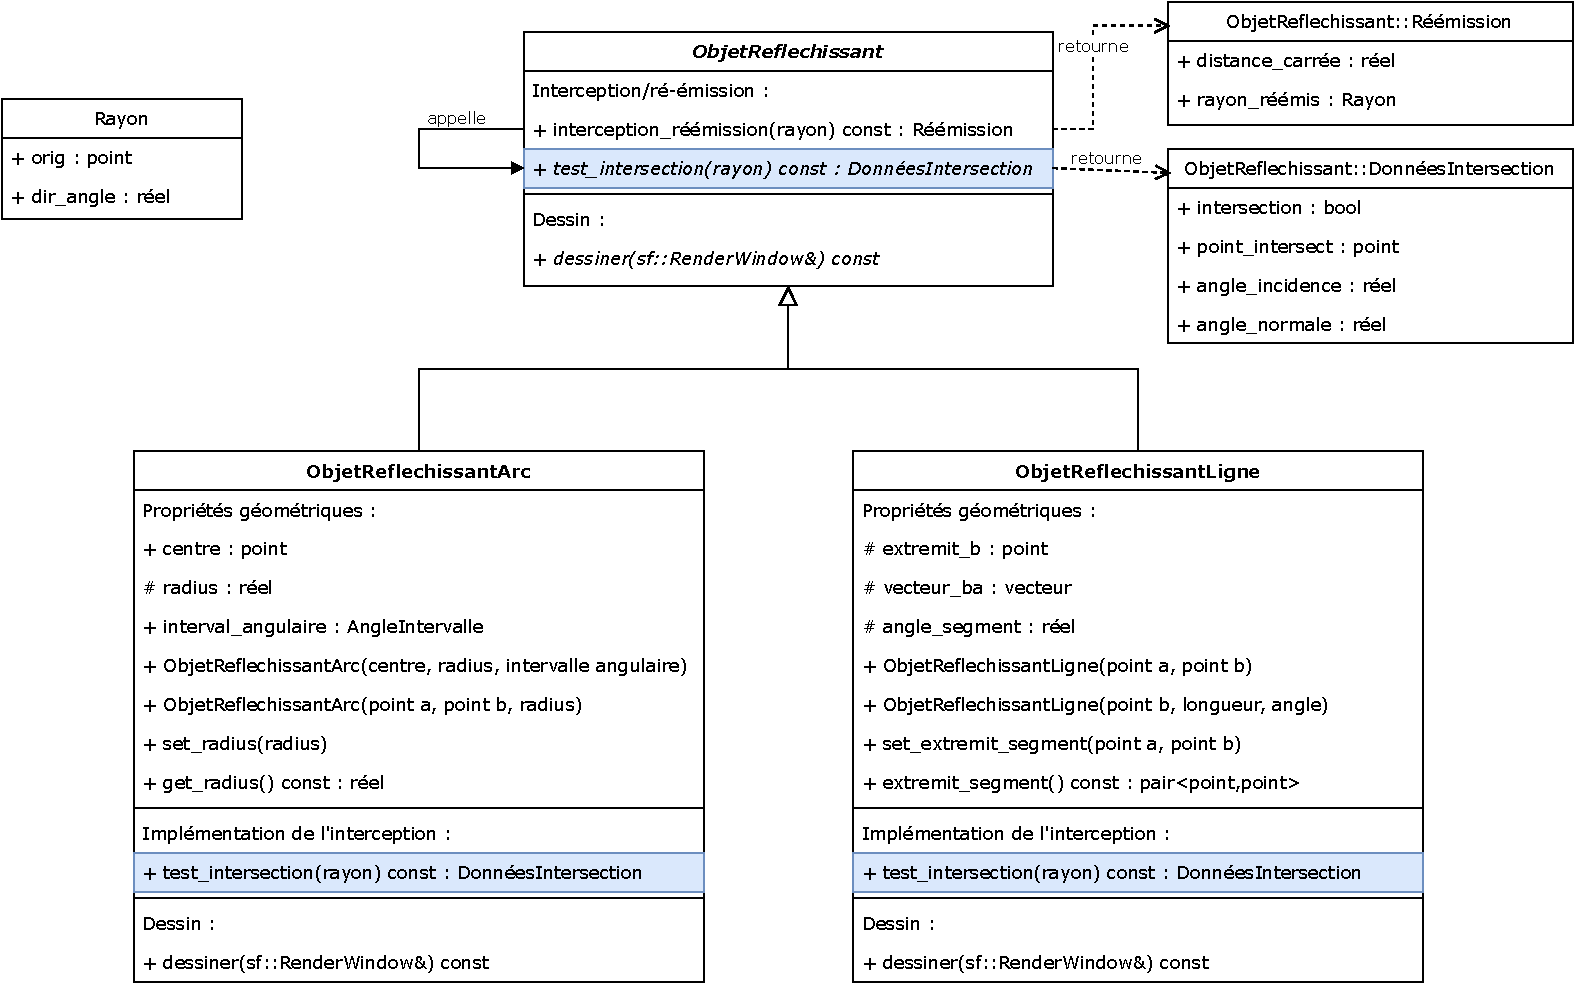
\includegraphics[width=\textwidth]{TD5/class-diagram.pdf}
  \caption{Diagramme de classes partiel. \texttt{ObjetReflechissantArc} et \texttt{ObjetReflechissantLigne} héritent de la classe abstraite \texttt{ObjetReflechissant}, et surchargent les méthodes virtuelles \inline{dessiner} et \inline{essai_interception} (surligné en bleu). On remarque que les classes ou méthodes abstraites sont en italique. Les attributs \inline{public} sont préfixés d'un +, et les \inline{protected} par un \#.}
  \label{fig:diagclasses1}
\end{figure}

\subsubsection{La classe de base}

\begin{enumerate}

  \item Créez la classe de base \texttt{ObjetReflechissant}. Comme il n'y a aucun attributs, aucun construteur n'a besoin d'être défini, même si c'est une bonne pratique que l'en définir un pour être explicite. Comme il s'agit d'une classe virtuelle, il faut déclarer un destructeur (\inline{virtual}, ici ne faisant rien). On supprimera aussi l'opérateur d'assignation car il ne servira pas.

\begin{correction}
\begin{minted}[fontsize=\footnotesize]{c++}
class ObjetReflechissant {
public:
  
  ObjetReflechissant () {}
  ObjetReflechissant& operator= (const ObjetReflechissant&) = delete;
  ObjetReflechissant (const ObjetReflechissant&) {}
  virtual ~ObjetReflechissant () {}
}
\end{minted}
\end{correction}

  \item Déclarez la méthode \inline{void dessiner (sf::RenderWindow&) const} comme abstraite, c'est-à-dire virtuelle pure. La classe sera donc aussi abstraite.

  \item Faites de même pour la méthode virtuelle \inline{test_intersection}. Cette méthode renvoie un objet
  \begin{minted}[samepage]{c++}
  struct DonnéesIntersection {
    bool intersection;
    Point2 point_intersect; // Point d'intersection
    double angle_incidence; // Angle d'incidence (angle du rayon à la normale)
    double angle_normale; // Angle absolu du vecteur normal à la courbe
  };
  \end{minted}
  que l'on pourra déclarer au sein de la classe \texttt{ObjetReflechissant}.\footnote{Il est possible que la version du compilateur que vous utilisez ne supporte pas encore les caractères accentuées dans le code. Dans ce cas, supprimez simplement les accents.}

  \item Déclarez et implémentez la méthode \inline{Réémission interception_réémission (const Rayon& ray) const}. Cette méthode appelle \inline{test_intersection} et un objet \inline{Réémission} contenant deux champs :
  \begin{itemize}
    \item \inline{double distance_carrée}, qui est la distance au carré\footnote{Quand il s'agit de comparer des distances, autant travailler avec les distances au carré, ça évite un coûteux appel à \inline{sqrt()}.} entre l'origine du rayon et l'éventuel point d'intersection, et \inline{Inf} si il n'y a pas interception (c'est l'élément neutre de la recherche de minimum).
    \item \inline{Rayon rayon_réémis}, qui est l'éventuel rayon réfléchi; on pourra y assigner \inline{Rayon::rayon_invalide()} si il n'y a pas interception.
  \end{itemize}
  Il se trouve que pour éviter la ré-interception immédiate d'un rayon émis par la même surface, dûe à des erreurs d'arrondi, il est nécessaire de rajouter une distance minimale (par exemple $10^{-6}$) en dessous de laquelle on dit qu'il n'y a pas intersection (on renvoie \inline{Inf}).
  Si il y a interception du rayon, le rayon ré-émis suivra la loi de la réflection : \emph{par rapport à la normale, l'angle de réflection est égal à l'angle d'incidence}. En terme d'angles absolus par rapport à l'horizontale, on a alors $$\alpha_\text{r} = \theta_\text{n} - i$$ où $i$ est l'angle d'incidence (angle relatif depuis la normale dans le sens trigonométrique), $\alpha_\text{r}$ est l'angle absolu du rayon réfléchi et $\theta_\text{n}$ est l'angle absolu de la normale à la surface.

\end{enumerate}

\begin{correction}

\subsubsection*{Fichier \filename{ObjetReflechissantBase.h}}

\begin{minted}[fontsize=\footnotesize,mathescape,xrightmargin=0.5cm,xleftmargin=0.5cm]{c++}
#ifndef _OBJBASE_H_
#define _OBJBASE_H_

#include "Util.h"
#include <SFML/Graphics/RenderWindow.hpp>

//-----------------------------------------------------------------------------------------------
// Classe de base des objets réfléchissants, où la surface de réflection est une ligne.
// Déclare l'interface commune utilisée lors de la propagation (interception puis ré-émission)
// des rayons, et l'affichage. Un ObjetReflechissant est capable de tester l'interception
// d'un rayon avec `interception_réémission` et, le cas échéant, de ré-émettre le rayon.
// Il est aussi capable de se dessiner dans une fenêtre SFML avec `dessiner`.

class ObjetReflechissant {
public:
  
  ObjetReflechissant () {}
  ObjetReflechissant& operator= (const ObjetReflechissant&) = delete;
  ObjetReflechissant (const ObjetReflechissant&) {}
  virtual ~ObjetReflechissant () {}

  // L'objet intercepte-t-il le rayon ? Si oui, donne la distance géométrique au carré
  //  parcourue par le rayon depuis son point d'émission ainsi qu'un rayon réfléchi.
  //  Sinon, renvoie Inf.
  struct Réémission {
    double distance_carrée;
    Rayon rayon_réémis;
  };
  Réémission interception_réémission (const Rayon& ray) const;
  
  // Méthode de test d'intersection, à surcharger dans les classes filles en fonction de la géométrie.
  struct DonnéesIntersection {
    bool intersection;
    Point2 point_intersect; // Point d'intersection
    double angle_incidence; // Angle d'incidence (angle du rayon à la normale)
    double angle_normale; // Angle absolu du vecteur normal à la courbe (par rapport à l'horizontale)
  };
  virtual DonnéesIntersection test_intersection (const Rayon& ray) const = 0;

  // Rendu graphique de l'objet, à surcharger dans les classes filles.
  virtual void dessiner (sf::RenderWindow& window) const = 0;
};

#endif
\end{minted}

\subsubsection*{Fichier \filename{ObjetReflechissantBase.cpp}}

\begin{minted}[fontsize=\footnotesize,mathescape,xrightmargin=0.5cm,xleftmargin=0.5cm]{c++}
#include "ObjetReflechissantBase.h"
#include <cmath>

ObjetReflechissant::Réémission ObjetReflechissant::interception_réémission (const Rayon& ray) const
{
  // Appel de la méthode de test d'intersection dépendant de la géométrie
  DonnéesIntersection isect = test_intersection(ray);

  if (isect.intersection) {
    double dist2 = (ray.orig - isect.point_intersect).norm2();
    // on introduit une distance minimale qu'un rayon peut parcourit avant d'être intercepté
    // par une courbe pour éviter qu'un objet ré-intercepte immédiatement le rayon qu'il vient
    // d'émettre, ce qui arriverait souvent en simple précision
    if (dist2 < 1e-10) {
      return {Inf, Rayon::rayon_invalide()};
    }
    else {
      Réémission r;
      // Loi de la réflection : i_refl = i par rapport à la normale
      r.rayon_réémis.orig = isect.point_intersect;
      r.rayon_réémis.dir_angle = isect.angle_normale - isect.angle_incidence;
      r.distance_carrée = dist2;
      return r;
    }
  }
  else {
    return {Inf, Rayon::rayon_invalide()};
  }
}
\end{minted}

\end{correction}

\subsubsection{La classe pour les segments}

Notre première géométrie de surface sera le segment, implémentée par la classe \inline{ObjetReflechissantLigne}. Pour les calculs d'intersection, le segment $AB$ sera plus efficacement représenté par la paire $(B,\vec{BA})$. On gardera aussi en mémoire l'angle à l'horizontale du segment pour accélérer les calculs. Ainsi, notre classe \inline{ObjetReflechissantLigne} possèdera trois attributs privés :
\begin{itemize}
  \item \inline{Point2 extremit_b}
  \item \inline{Vec2 vecteur_ba}
  \item \inline{double angle_segment}
\end{itemize}

\begin{figure}[H]
  \centering
  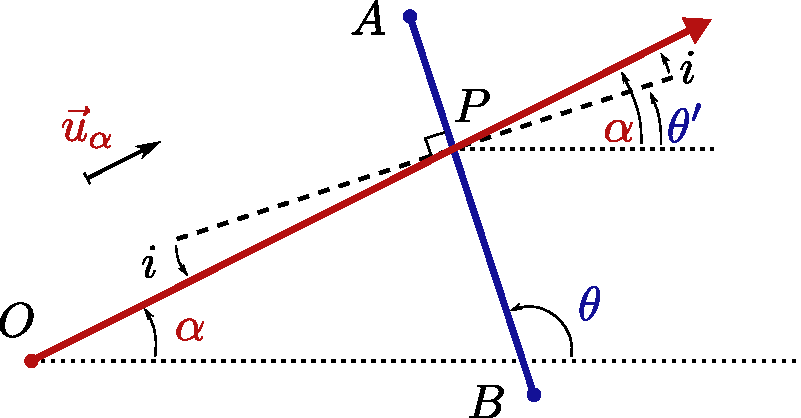
\includegraphics[width=0.4\textwidth]{TD5/isect-seg-dd.pdf}
  \caption{Schéma de l'interception d'un rayon (origine $O$, angle $\alpha$) par un segment $AB$.}
  \label{fig:isect-seg-dd}
\end{figure}

Comment tester si un rayon $(O,\alpha)$ intersecte le segment $AB$ ? L'ensemble des points du segment peut être paramétré ainsi :
$$s\,A + (1-s)\,B \quad \text{pour} \quad s \in [0;1]$$

Aussi, l'ensemble des points de la demi-droite d'origine $O$ portée par $\vec{u}_{\alpha}=(x_\alpha,y_\alpha)=(\cos \alpha, \sin \alpha)$, représentant le rayon, peut être paramétré ainsi :
$$O + t\,\vec{u}_{\alpha} \quad \text{pour} \quad t \in [0; \infty [$$

On a donc intersection lorsque ces deux ensembles ont un point en commun, c'est-à-dire lorsque $\exists\,s_{\text{i}} \in [0; 1], t_{\text{i}} \in [0; \infty[$ tels que
\begin{equation*}
  \quad A\,s_{\text{i}} + (1-s_{\text{i}})\,B = O + t_{\text{i}}\,\vec{u}_{\theta}
  \quad \Leftrightarrow \quad
  \overrightarrow{BA}\,s_{\text{i}} + t_{\text{i}}\,\vec{u}_{\alpha} = \overrightarrow{BO}
  \quad \Leftrightarrow \quad
  \left[\begin{array}{cc}
     x_A - x_B & - x_{\alpha}\\
     y_A - y_B & - y_{\alpha}
   \end{array}\right]  \left[\begin{array}{c}
     s_{\text{i}}\\
     t_{\text{i}}
   \end{array}\right] = \left[\begin{array}{c}
     x_O - x_B\\
     y_O - y_B
   \end{array}\right]
\end{equation*}

En ignorant le cas où le segment et la demi-droite sont parallèles, il
suffit de résoudre ce système linéaire. Si $s \notin [0, 1]$ ou si $t < 0$,
alors il n'y a pas intersection. Sinon, le point d'intersection est $P = O + t_{\text{i}}\,\vec{u}_{\alpha}$, et l'angle d'incidence est $i = \alpha - \theta'$, où $\theta = \angle \overrightarrow{B A}$ (attribut \inline{angle_segment}) et $\theta' = \theta - \frac{\pi}{2}$ (cf.\ figure \ref{fig:isect-seg-dd}). L'angle de la normale est $\theta_{\text{n}} = \theta' + \pi$. On pourra s'amuser à rapporter les valeurs numériques de ces angles aux intervalles usuels ($i\in[-\pi,\pi]$ par exemple), mais ce n'est pas nécessaire pour des simples réflections.\\

Nous sommes maintenant prêts à implémenter cette classe.

\begin{enumerate}

  \item Déclarez la classe \inline{ObjetReflechissantLigne}, héritant de la classe de base, et déclarez ses attributs géométriques.

  \item Mettez à disposition deux contructeurs :
  \begin{itemize}
    \item \inline{ObjetReflechissantLigne (Point2 a, Point2 b)} pour créer un segment d'extrémités \inline{a} et \inline{b}
    \item \inline{ObjetReflechissantLigne (Point2 b, double longueur, double angle)} pour créer un segment ayant une extrémité \inline{b}, une longueur donnée et un angle donné par rapport à l'horizontale
  \end{itemize}
  ainsi qu'un setter \inline{void set_extremit_segment (Point2 a, Point2 b)}. Optionnellement, mettez à disposition un getter \inline{std::pair<Point2,Point2> extremit_segment () const} renvoyant les deux points d'extrémité.

  \item En utilisant le raisonnement décrit ci-dessus, déclarez et implémentez la méthode virtuelle \inline{DonnéesIntersection test_intersection (const Rayon& rayon) const}, testant l'intersection du rayon \inline{rayon} avec le segment, et renvoyant un objet \inline{ObjetReflechissant::DonnéesIntersection} dont le champ \inline{bool intersection} indique si l'intersection a lieu ou non, et dont les trois autres champs, décrits dans la partie précédente, sont remplis lorsque c'est le cas.

  \item Il est maintenant temps de tester nos classes. Compilez vos deux fichiers \filename{.cpp} et réglez les éventuelles erreurs de syntaxe/compilation. Ensuite, créez un fichier \filename{main.cpp}, où est instancié un \inline{ObjetReflechissantLigne}. Compilez. Pourquoi, à votre avis, le compilateur vous empêche-t-il d'instancier cette classe ?

  \item Implémentez ce qu'il manque pour pouvoir instancier la classe...
\end{enumerate}

\begin{correction}

\subsubsection*{Fichier \filename{ObjetReflechissantLigne.h}}

\begin{minted}[fontsize=\footnotesize,mathescape,xrightmargin=0.5cm,xleftmargin=0.5cm]{c++}
#ifndef _OBJLIGNE_H_
#define _OBJLIGNE_H_

#include "ObjetReflechissantBase.h"

class ObjetReflechissantLigne : public ObjetReflechissant {
protected:
  Point2 extremit_b;
  Vec2 vecteur_ba;
  double angle_segment;  // angle (horizontale,a,b) gardé en cache pour optimisation

public:
  // Constructeurs et destructeur
  ObjetReflechissantLigne (Point2 a, Point2 b);
  ObjetReflechissantLigne (Point2 b, double longueur, double angle);
  ObjetReflechissantLigne (const ObjetReflechissantLigne& o);
  virtual ~ObjetReflechissantLigne () {}

  // Getter
  std::pair<Point2,Point2> extremit_segment () const;
  // Setter
  void set_extremit_segment (Point2 a, Point2 b);

  // Implémentation du test d'interception
  virtual DonnéesIntersection test_intersection (const Rayon& ray) const;

  // Dessin
  virtual void dessiner (sf::RenderWindow& window) const;
};

#endif
\end{minted}

\subsubsection*{Fichier \filename{ObjetReflechissantLigne.cpp}}

\begin{minted}[fontsize=\footnotesize,mathescape,xrightmargin=0.5cm,xleftmargin=0.5cm]{c++}
#include "ObjetReflechissantLigne.h"
#include <SFML/Graphics.hpp>
#include <cmath>
using namespace std;

void ObjetReflechissantLigne::set_extremit_segment (Point2 a, Point2 b) {
  vecteur_ba = a - b;
  extremit_b = b;
  angle_segment = atan2(vecteur_ba.y, vecteur_ba.x);
}

std::pair<Point2,Point2> ObjetReflechissantLigne::extremit_segment () const {
  return { extremit_b + vecteur_ba, extremit_b };
}

ObjetReflechissantLigne::ObjetReflechissantLigne (const ObjetReflechissantLigne& o)
  : ObjetReflechissant(o), extremit_b(o.extremit_b), vecteur_ba(o.vecteur_ba), angle_segment(o.angle_segment)
{}

ObjetReflechissantLigne::ObjetReflechissantLigne (Point2 a, Point2 b) {
  set_extremit_segment(a, b);
}

ObjetReflechissantLigne::ObjetReflechissantLigne (Point2 b, double longueur, double angle) :
  extremit_b(b),
  vecteur_ba(longueur * Vec2::u_angle(angle)),
  angle_segment(angle)
{}

// Test d'intersection du rayon sur le segment.
// Cas particulier d'alignement non pris en compte
//
ObjetReflechissant::DonnéesIntersection ObjetReflechissantLigne::test_intersection (const Rayon& ray) const {
  DonnéesIntersection isect;

  Vec2 u_rayon = Vec2::u_angle(ray.dir_angle);
  double s, t;
  mat22_sol(vecteur_ba.x, -u_rayon.x,
            vecteur_ba.y, -u_rayon.y,
            ray.orig.x - extremit_b.x, ray.orig.y - extremit_b.y,
            s, t);
  if ((0 <= s and s <= 1) and t >= 0) {
    isect.intersection = true;
    // point d'incidence
    isect.point_intersect = ray.orig + t * u_rayon;
    // angle d'incidence
    double alpha = angle_mod2pi_11(ray.dir_angle);
    double i = alpha - (angle_segment - M_PI/2);
    if (fabs(angle_mod2pi_11(i)) < M_PI/2) {
      isect.angle_normale = angle_segment + M_PI/2;
      isect.angle_incidence = i;
      // isect.sens_reg = true;
    } else {
      isect.angle_incidence = i - M_PI;
      if (isect.angle_incidence < -M_PI/2)
        isect.angle_incidence += 2*M_PI;
      isect.angle_normale = angle_segment - M_PI/2;
      // isect.sens_reg = false;
    }
    /* note : le code écrit ici sépare le cas d'un rayon arrivant sur une face
       ou l'autre du segment et rapport les angles modulo 2pi aux intervalles
       usuels; cela ne sert à rien pour une simple réflexion, mais ce code a
       initialement été écrit pour traiter des rayons en optique géométrique,
       avec réflexion et réfraction. */
  } else {
    isect.intersection = false;
  }
  return isect;
}

// Affichage
//
void ObjetReflechissantLigne::dessiner (sf::RenderWindow& window) const {
  auto [a,b] = extremit_segment();
  sf::VertexArray line (sf::Lines, 2);
  line[0] = sf::Vertex( coord_01_vers_fenetre(a), sf::Color::White );
  line[1] = sf::Vertex( coord_01_vers_fenetre(b), sf::Color::White );
  window.draw(line);
}
\end{minted}

\end{correction}

\subsubsection{Quelques tests}

Il est temps de tester notre classe, et en particulier le code d'interception, où les chances de faire une erreur est grande. Pour gagner du temps, on pourra partir du fichier \filename{main-modèle.cpp}, qui implémente une boucle d'affichage SFML avec une fenêtre \inline{window}. Un rayon \inline{traj0} y est déclaré, dont l'origine est contrôlable au clic de la souris (évènement SFML \inline{sf::Event::MouseButtonReleased}), et dont la direction suit la souris (évènement SFML \inline{sf::Event::MouseMoved}). Un objet \inline{ObjetReflechissantLigne obj} est aussi instancié. Renommez le fichier en \filename{main\_sec532.cpp}; on pourra exécuter \texttt{make billard\_sec532} pour compiler et exécuter le programme.\\

Pour tester le code d'interception, appellez \inline{ObjetReflechissant::test_intersection} sur le rayon, et si il y a intersection, dessinez une ligne entre l'origine du rayon et le point d'intersection (par exemple en rouge avec \inline{sf::Color::Red}). De plus, dessinez toujours le segment avec \inline{ObjetReflechissant::dessin}.

\begin{correction}
Il suffit d'ajouter le code suivant à la place de \inline{// ...} :
\begin{minted}[fontsize=\footnotesize,mathescape,xrightmargin=0.5cm,xleftmargin=0.5cm]{c++}
ObjetReflechissant::DonnéesIntersection isect = obj.test_intersection(traj0);

if (isect.intersection) {
  sf::VertexArray line (sf::Lines, 2);
  line[0] = sf::Vertex( coord_01_vers_fenetre( traj0.orig ), sf::Color::Red );
  line[1] = sf::Vertex( coord_01_vers_fenetre( isect.point_intersect ), sf::Color::Red );
  window.draw(line);
}

obj.dessiner(window);
\end{minted}
\end{correction}

On doit alors obtenir le résultat suivant :
\begin{center}
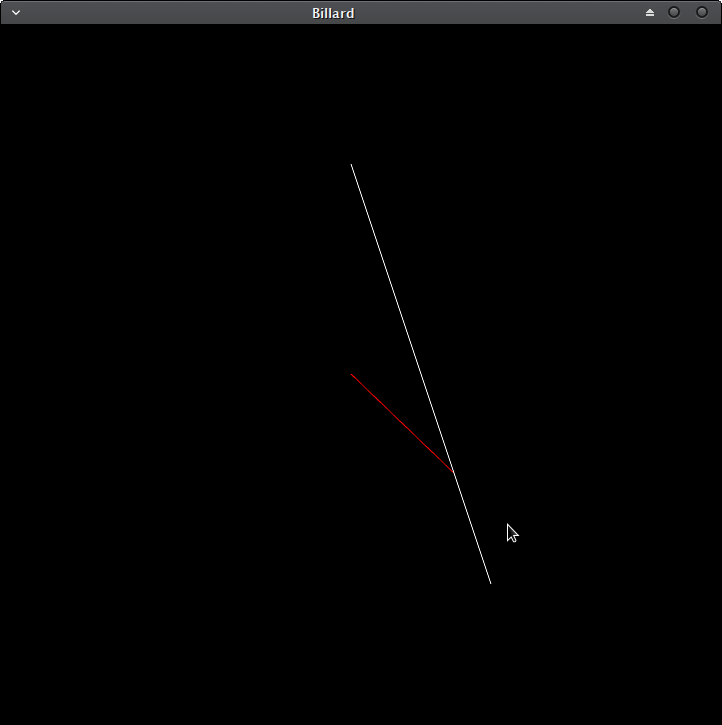
\includegraphics[width=0.5\textwidth]{TD5/test-intersection.png}
\end{center}

\subsubsection{La classe pour les arcs de cercle}

Notre seconde géométrie de surface sera l'arc de cercle, implémentée par la classe \inline{ObjetReflechissantArc}. Elle possèdera naturellement trois attributs :
\begin{itemize}
  \item \inline{Point2 centre}
  \item \inline{AngleIntervalle interval_angulaire}
  \item \inline{double radius}, le rayon de l'arc de cercle, que l'on déclarera privé pour empêcher l'utilisateur de le rendre négatif; il faudra donc ajouter un setter et getter pour le rayon.
\end{itemize}

\begin{enumerate}

  \item Déclarez la classe \inline{ObjetReflechissantArc}, héritant de la classe de base, et déclarez ses attributs géométriques. Définissez un constructeur initialisant ces trois attributs, en vérifiant si le rayon est valide, et lançant une exception si ce n'est pas le cas :
  \begin{minted}[xleftmargin=0.5cm]{c++}
  if (radius <= 0.f)
    throw std::domain_error("ObjetReflechissantArc : le rayon ne peut être négatif.");
  \end{minted}
  Optionnellement (ça ne servira pas dans la suite), mettez à disposition un setter et getter pour le rayon de l'arc de cercle.

  \item Déclarez et implémentez la méthode virtuelle \inline{void dessiner (sf::RenderWindow& window) const}. Il n'y a pas de moyen direct de dessiner un arc de cercle avec la SFML. On pourra simplement dessiner un arc de polygone régulier qui, si le nombre de points est suffisant, est indistinguable d'un arc de cercle :
  \begin{minted}[xleftmargin=0.5cm]{c++}
  int npoints = std::max<int>(7, radius * 400 * interval_angulaire.longueur());
  sf::VertexArray lines (sf::LineStrip, npoints+1);
  for (int k = 0; k <= npoints; k++) {
    double theta = interval_angulaire.beg()
                + interval_angulaire.longueur() * (double) k / npoints;
    lines[k] = sf::Vertex(
      coord_01_vers_fenetre( centre + radius * Vec2::u_angle(theta) ),
      sf::Color::White
    ); 
  }
  window.draw(lines);
  \end{minted}

  \item Déclarez la méthode virtuelle \inline{DonnéesIntersection test_intersection (const Rayon& rayon) const}. Le test d'intersection entre une demi-droite et un arc de cercle est plus complexe à calculer et plus sujet à erreurs que pour un segment. Les plus téméraires pourront le faire eux mêmes à l'aide des notes dans \filename{intersection-demi-droite-cercle.pdf}. Les autres pourront utiliser le code suivant :
  \begin{minted}[fontsize=\footnotesize,mathescape,xleftmargin=0.5cm]{c++}
  ObjetReflechissant::DonnéesIntersection ObjetReflechissantArc::test_intersection (const Rayon& ray) const {
    Vec2 oc = centre - ray.orig;
    double b = !oc / radius;  // $d/R$
    double base_ang = atan2(oc.y, oc.x);
    // angles relatifs à l'axe $OC$ :
    double alpha = angle_mod2pi_11( ray.dir_angle - base_ang );
    AngleIntervalle thetaAB = interval_angulaire + -base_ang;
    // intersection avec le cecle si en dessous de l'angle critique
    double y = b * sin(alpha);
    if ( (b > 1+1e-10 and abs(alpha) >= M_PI/2) or abs(y) > 1 )
      return DonnéesIntersection{false};
    // angles repérant les points d'intersection avec le cercle
    double arcsiny = asin(y);
    double theta1 = alpha - arcsiny + M_PI,
          theta2 = alpha + arcsiny;
    double theta_incidence;
    /// si on est bien sur notre arc de cercle :
    DonnéesIntersection isect;
    // $\theta_1$ n'est accessible que si la rayon vient de l'extérieur ($b>1$);
    // on vérifie qu'il est bien dans l'intervalle angulaire de l'arc de cercle thetaAB
    if ( b > 1+1e-10 and thetaAB.inclus(theta1) ) {
      // isect.sens_reg = true; // ext vers int du cercle
      theta_incidence = theta1 + base_ang;
      isect.angle_normale = theta_incidence;
      isect.angle_incidence = M_PI - theta1 + alpha; // c'est un angle relatif, pas besoin de base_ang
    }
    // test de $\theta_2$ pour $b<1$ ou si $\theta_1$ a échoué pour $b>1$
    else if ( thetaAB.inclus(theta2) ) {
      // isect.sens_reg = false; // int vers ext du cercle
      theta_incidence = theta2 + base_ang;
      isect.angle_normale = theta_incidence + M_PI; // normale vers l'intérieur du cercle
      isect.angle_incidence = alpha - theta2;
    }
    else
      return DonnéesIntersection{false};
    // calcul du point d'incidence
    isect.point_intersect = centre + radius * Vec2::u_angle(theta_incidence);
    isect.intersection = true;
    return isect;
  }
  \end{minted}

  \item Testez le code d'interception comme ci-dessus, en remplaçant le segment par, par exemple, \inline{ObjetReflechissantArc( Point2{0.3,0.6}, 0.2, AngleIntervalle(1,-2) )}. On n'oublira pas de modifier le \filename{Makefile} pour que \filename{ObjetReflechissantArc.cpp} soit compilié et lié à \filename{main\_sec532.o}.

\end{enumerate}

\subsection{Implémentation du billard}

Pour le moment, nous n'avons manipulé qu'un seul objet. Il est temps de construire une scène composée de multiples objets et d'exploiter le polymorphisme. L'idéal serait de créer une classe \inline{Scene}, mais laissons ça pour la partie optionnelle du TD.\\

Nous allons stocker tous les objets de la scène dans un \inline{std::vector<ObjetReflechissant*>}. Il est crucial de ne \emph{pas} stocker directement des \inline{ObjetReflechissant} par valeur, comme on le ferait avec \inline{std::vector<ObjetReflechissant>}, car un tel conteneur ne pourrait pas stocker les objets d'un type différent, en l'occurence \inline{ObjetReflechissantLigne} et \inline{ObjetReflechissantArc} ! Comme nous voulons stocker des objets de types différents, comme les listes en Python, il est nécessaire de le faire indirectement en \cpp, c'est-à-dire à travers des pointeurs\footnote{Une référence n'étant pas un vrai objet en mémoire, il n'est pas possible de déclarer un tableau de références}. Nous pouvons utiliser soit
\begin{itemize}
  \item des pointeurs nus \inline{ObjetReflechissant*}, comme vous connaissez bien, qui nécessitent allocation (\inline{new ObjetReflechissantXXX(/*arguments du constructeurs*/)}) et désallocation (\inline{delete}) à la main
  \item les \emph{pointeurs automatiques} du \cpp, par exemple \inline{std::shared_ptr<ObjetReflechissant>}, qui \inline{delete} automatiquement dans leur destructeur; un tel pointeur automatique (et son objet) peut être créé par \inline{std::make_shared<ObjetReflechissantXXX>(/*arguments du constructeurs*/)}, où les arguments sont ceux du constrcuteur de \inline{ObjetReflechissantXXX}.
\end{itemize}
On restera sur des pointeurs nus par facilité, mais n'hésitez pas à adopter les pointeurs automatiques.

% Quelques mots sur l'upcasting et le polymorphisme d'un pointeur sur la classe de base ?

\begin{enumerate}

  \item Copiez le précédent \filename{main.cpp} en un \filename{main\_sec533.cpp} (on pourra alors faire \texttt{make billard\_sec533}). Déclarez-y un tableau de pointeurs sur la classe de base, et remplissez-le de quelques objets (quelques lignes et quelques arcs de cercle). N'oubliez pas de les \inline{delete} à la fin du \inline{main()}.

\begin{correction}
\begin{minted}[fontsize=\footnotesize]{c++}
int main () {

  // Génération de nombres aléatoires entre 0 et 1
  std::default_random_engine generator;
  std::uniform_real_distribution<double> distribution(0.0,1.0);
  auto rand01 = [&] () -> double {
    return distribution(generator);
  };

  // Conteneur des objets de la scène
  std::vector<ObjetReflechissant*> objets;

  for (int i = 0; i < 10; ++i) {
    // Quelques segments aléatoires
    objets.push_back(new ObjetReflechissantLigne(
      Point2{rand01(),rand01()},
      0.08,
      rand01()*2*M_PI
    ));
    // Quelques arcs aléatoires
    objets.push_back(new ObjetReflechissantArc(
      Point2{rand01(),rand01()},
      0.04,
      AngleIntervalle(+M_PI/2,-M_PI/2)+2*M_PI*rand01()
    ));
  }

  /* Boucle principale */
  while (window.isOpen()) {
    /* ... */
  }

for (ObjetReflechissant* obj : objets) 
  delete obj;
\end{minted}
Bien que \inline{obj} est un pointeur sur la classe de base, et que la bonne surcharge à appeler ne peut donc pas être connue au moment de la compilation, comme la méthode \inline{dessiner} est virtuelle, au moment de l'exécution, la bonne surcharge sera sélectionné en fonction du vrai type du l'objet. C'est le polymorphisme.
\end{correction}

  \item Dans la boucle principale, affichez tous les objets de la scène avec \inline{ObjetReflechissant::dessin}. Compilez et testez. En quoi exploitons-nous le polymorphisme ?

\begin{correction}
On ne peut pas faire plus simple :
\begin{minted}[fontsize=\footnotesize]{c++}
for (ObjetReflechissant* obj : objets) 
  obj->dessiner(window);
\end{minted}
Bien que \inline{obj} est un pointeur sur la classe de base, et que la bonne surcharge à appeler ne peut donc pas être connue au moment de la compilation, comme la méthode \inline{dessiner} est virtuelle, au moment de l'exécution, la bonne surcharge sera sélectionné en fonction du vrai type du l'objet. C'est le polymorphisme.
\end{correction}

  \item Créez une fonction \inline{interception_réémission} prennant en argument le tableau d'objets, un rayon, et renvoyant une \inline{std::pair<ObjetReflechissant*,Rayon>}. Cette fonction appellera la méthode\linebreak\inline{ObjetReflechissant::interception_réémission} sur chaque objet de la scène et choisira le premier objet sur le trajet du rayon, s'il existe. Le premier élément de la paire sera un pointeur sur cet objet (\inline{nullptr} si il n'y a aucune interception), et le deuxième élément sera la rayon éventuellement ré-émis.

\begin{correction}
C'est une simple recherche de minimum :
\begin{minted}[fontsize=\footnotesize]{c++}
std::pair<ObjetReflechissant*,Rayon> interception_réémission (
  const std::vector<ObjetReflechissant*>& objets,
  Rayon rayon_in
)
{
  double dist2_min = Inf;
  Rayon rayon_réémis;
  ObjetReflechissant* obj_intercept = nullptr;
  
  for (ObjetReflechissant* obj : objets) {
    ObjetReflechissant::Réémission r = obj->interception_réémission(rayon_in);
    if (r.distance_carrée < dist2_min) {
      dist2_min = r.distance_carrée;
      rayon_réémis = r.rayon_réémis;
      obj_intercept = obj;
    }
  }

  return { obj_intercept, rayon_réémis };
}
\end{minted}
On remarque que le tableau d'objets est passé par référence (constante) : c'est toujours une bonne pratique pour les gros objets de ce type pour éviter les copies inutiles.
\end{correction}

  \item Dans la boucle principale, écrivez un code effectuant la propagation de la trajectoire et son dessin parmis les objets de la scène. Vous pouvez déclarer un \inline{Rayon traj_courant}, qui vaut initialement \inline{traj0} (le rayon dont la direction est déterminée par la position de la souris), et à qui vous assignez tour-à-tour le rayon ré-émis par le premier objet interceptant le rayon précédent. Faites une boucle qui s'arrête lorsque le rayon n'est intercepté par aucun objet. À chaque itération, dessinez le segment entre l'origine du rayon courant et l'origine du rayon ré-émis. Enfin, après la sortie de boucle, dessinez la demi droite représentant le rayon non intercepté; on peut se permettre de seulement dessiner un second point qui est en dehors de la fenêtre, par exemple comme ceci :
  \begin{minted}[fontsize=\footnotesize]{c++}
  sf::VertexArray line (sf::Lines, 2);
  line[0] = sf::Vertex( coord_01_vers_fenetre( traj_courant.orig ), sf::Color::Red );
  Point2 far_away = traj_courant.orig + 10 * Vec2::u_angle(traj_courant.dir_angle);
  line[1] = sf::Vertex( coord_01_vers_fenetre( far_away ), sf::Color::Red );
  window.draw(line);
  \end{minted}
  Note : pour accéder aux éléments d'une \inline{std::pair<A,B> p}, utilisez \inline{p.first} et \inline{p.second}, ou utilisez la syntaxe suivante : \inline{auto [a,b] = p;}

\begin{correction}
\begin{minted}[fontsize=\footnotesize]{c++}
// Contruction de la trajectoire par propagation du rayon traj0

Rayon traj_courant = traj0;

while (true) {

  // Interception par le premier objet sur le chemin du rayon courant
  auto [obj,traj_next] = interception_réémission(objets, traj_courant);
  if (obj == nullptr) 
    break;

  // Dessin du segment de trajectoire
  sf::VertexArray line (sf::Lines, 2);
  line[0] = sf::Vertex( coord_01_vers_fenetre( traj_courant.orig ), sf::Color::Red );
  line[1] = sf::Vertex( coord_01_vers_fenetre( traj_next.orig ), sf::Color::Red );
  window.draw(line);
  
  traj_courant = traj_next;
}

// Dessin de la demi-droite finale
sf::VertexArray line (sf::Lines, 2);
line[0] = sf::Vertex( coord_01_vers_fenetre( traj_courant.orig ), sf::Color::Red );
Point2 far_away = traj_courant.orig + 10 * Vec2::u_angle(traj_courant.dir_angle);
line[1] = sf::Vertex( coord_01_vers_fenetre( far_away ), sf::Color::Red );
window.draw(line);
\end{minted}
\end{correction}

  \item Compilez et testez. Vous devriez avoir un résultat semblable à la capture d'écran de la partie introductive.

  \item On peut maintenant explorer les trajectoires d'un vrai billard, c'est-à-dire une surface fermée. Pour cela, modifiez d'abord la boucle de propagation pour qu'elle s'arrête au bout d'un nombre déterminé de ré-émissions, par exemple 1000. Pour y voir plus clair, on pourra réduire l'opacité des segments de la trajectoire : un rouge opaque à 10\% est obtenu avec \inline{sf::Color(255,0,0,25)}. Puis, pour les surfaces, on pourra prendre un billard formé de deux demi-cercles non-concentriques et de deux segments fermant le billard :
  \begin{minted}[fontsize=\footnotesize]{c++}
  objets.push_back(new ObjetReflechissantLigne( Point2{0.5-z,0.2}, Point2{0.5+z,0.2} ));
  objets.push_back(new ObjetReflechissantLigne( Point2{0.5-z,0.8}, Point2{0.5+z,0.8} ));
  objets.push_back(new ObjetReflechissantArc( Point2{0.5+z,0.5}, 0.3, AngleIntervalle(+M_PI/2,-M_PI/2) ));
  objets.push_back(new ObjetRelechissantArc( Point2{0.5-z,0.5}, 0.3, AngleIntervalle(-M_PI/2,+M_PI/2) ));
  \end{minted}
  paramétré par $z$, réel de signe quelconque. Explorez la différence entre $z=0$, $z>0$ et $z<0$. Pour $z>0$, il s'agit du fameux \emph{stade de Bunimovich} :
  \begin{center}
  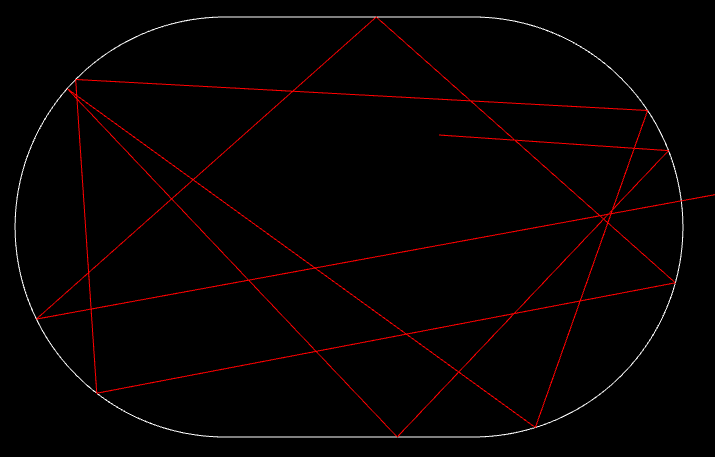
\includegraphics[height=20em]{TD5/bunimovich-stadium.png}
  \end{center}

\begin{correction}
L'ensemble est présent dans le fichier \filename{main\_sec533.cpp}.
\end{correction}

\end{enumerate}

\section{[Bonus] Exploration de l'espace des phases}

Cette partie du TD est optionnelle. Il s'agit d'extraire et d'afficher des informations pertinentes sur la dynamique du système. On peut déjà dire beaucoup de choses en regardant les trajectoires dans l'espace des phases.

\subsection{Une classe pour la scène}

Avant d'explorer l'espace des phases, nettoyons le \filename{main.cpp} en créant une classe \inline{Scene}. Cette classe stockera tous les éléments de la scène, et implémentera les routines de propagation des trajectoires.\\

Le header \filename{Scene.h} est fourni pour gagner du temps. On remarque :
\begin{itemize}
  \item Le stockage polymorphique des objets de la scène avec \inline{std::vector<ObjetReflechissant*> objets}, comme dans la partie précédente
  \item L'allocation des objets est faite par la classe \inline{Scene} elle-même dans une méthode \inline{template <class ObjT, typename... Args> ObjT& créer_objet (Args&& ...args)}, dont le prototype peut effrayer. Il s'agit d'une méthode template, dont le premier argument template \inline{ObjT} est le type de l'objet à créer. Elle prend un nombre arbitraire d'arguments, et passe simplement ces arguments au contructeur de \inline{ObjT} en écrivant \inline{ObjT(std::forward<Args>(args)...)}, similaire au \texttt{**kwargs} en Python. L'objet nouvellement créé est inséré dans le \inline{std::vector}. Enfin, la méthode renvoie une référence sur l'objet créé au cas où l'utilisateur veut manipuler l'objet.
  \item La désallocation des objets est automatique grâce à l'appel du destructeur. On pourrait se passer totalement du destructeur si on utilisait des pointeurs automatiques à la place de pointeurs nus.
\end{itemize}

\vspace{1em}
En déportant simplement le code des parties précédentes dans la classe \inline{Scene}, implémentez les méthodes \inline{interception_réémission} et \inline{dessiner_scene}.\\

On va séparer le calcul de la trajectoire et son affichage. Écrivez la méthode\\
\inline{  std::vector<Rayon> propagation_trajectoire (Rayon traj0, size_t limite_taille)}\\
qui utilise \inline{Scene::interception_réémission} pour contruire la trajectoire (avec une limite de réflexions \inline{limite_taille}), et qui renvoie la trajectoire sous forme d'un tableau des rayons successifs\footnote{Ce n'est pas la représentation la plus élégante, mais ça contient toutes les informations sur la trajectoire}. Écrivez ensuite la méthode\\
\inline{  std::vector<Rayon> propagation_trajectoire (Rayon traj0, size_t limite_taille, sf::RenderWindow&, sf::Color couleur_traj)}\\
qui appelle la méthode précedente pour calculer la trajectoire, dessine en plus la trajectoire (réutilisez le code de la partie précédente) avec une certaine couleur \inline{couleur_traj} dans une fenêtre SFML, et renvoie la trajectoire.

\begin{correction}
\begin{minted}[fontsize=\footnotesize]{c++}

// Caclul d'une trajectoire sur la scène : récursion de l'interception/ré-émission
// Renvoie la trajectoire sous forme d'un tableau de rayons
//
std::vector<Rayon> Scene::propagation_trajectoire (Rayon rayon, size_t limite_taille) const {
  std::vector<Rayon> traj;
  // std::vector::reserve permet de pré-allouer de la mémoire, et évite ainsi
  // les éventuels coûteux redimentionnements lors des push_pack successifs
  traj.reserve(limite_taille+1);

  while (true) {
    traj.push_back(rayon);
    if (traj.size() > limite_taille) 
      break;
    auto p = this->interception_réémission(rayon);
    if (p.first == nullptr)
      break;
    rayon = p.second;
  }

  return traj;
}

// Caclul d'une trajectoire sur la scène et affichage de la trajectoire
//  dans la fenêtre window avec la couleur couleur_traj
//
std::vector<Rayon> Scene::propagation_trajectoire (
  Rayon traj0,
  size_t limite_taille,
  sf::RenderWindow& window,
  sf::Color couleur
) const
{
  // Calcul de la trajectoire
  std::vector<Rayon> traj = propagation_trajectoire(traj0, limite_taille);

  // Dessin des rayons
  sf::VertexArray line (sf::Lines, 2);
  for (size_t i = 0; i < traj.size()-1; ++i) {
    line[0] = sf::Vertex( coord_01_vers_fenetre( traj[i].orig ), couleur );
    line[1] = sf::Vertex( coord_01_vers_fenetre( traj[i+1].orig ), couleur );
    window.draw(line);
  }
  // Dessin du dernier rayon, non intercepté, allant à l'infini (ici = 10)
  const Rayon& last_rayon = traj.back();
  Point2 far_away = last_rayon.orig + 10 * Vec2::u_angle(last_rayon.dir_angle);
  line[0] = sf::Vertex( coord_01_vers_fenetre( last_rayon.orig ), couleur );
  line[1] = sf::Vertex( coord_01_vers_fenetre( far_away ), couleur );
  window.draw(line);

  return traj;
}
\end{minted}
\end{correction}

Enfin, ré-écrivez le \inline{main()} de la section précédente dans \inline{main_sec541.cpp} (on pourra faire \texttt{make billard\_sec541}) en utilisant la classe \inline{Scene} à la place du tableau d'objets et du code de propagation et d'affichage. Pour la création de notre billard, on pourra utiliser le code suivant :
\begin{minted}[fontsize=\footnotesize]{c++}
  auto& L1 = scene.créer_objet<ObjetReflechissantLigne>( Point2{0.5,0.2}, Point2{0.5,0.2} );
  auto& L2 = scene.créer_objet<ObjetReflechissantLigne>( Point2{0.5,0.8}, Point2{0.5,0.8} );
  auto& A1 = scene.créer_objet<ObjetReflechissantArc>( Point2{0.5,0.5}, 0.3, AngleIntervalle(+M_PI/2,-M_PI/2) );
  auto& A2 = scene.créer_objet<ObjetReflechissantArc>( Point2{0.5,0.5}, 0.3, AngleIntervalle(-M_PI/2,+M_PI/2) );

  auto modifier_billard = [&] (double z) {
    L1.set_extremit_segment( Point2{0.5-z,0.2}, Point2{0.5+z,0.2} );
    L2.set_extremit_segment( Point2{0.5-z,0.8}, Point2{0.5+z,0.8} );
    A1.centre = Point2{0.5+z,0.5};
    A2.centre = Point2{0.5-z,0.5};
  };
  double z = +0.081;
  modifier_billard(z);
\end{minted}
Une nouvelle syntaxe apparait : il s'agit des "fonctions lambda", qui ne sont rien d'autre que des fonctions que l'on peut déclarer n'importe où (comme les fonctions en Python) et stocker dans une variable de type \inline{std::function}, ici \inline{modifier_billard}. Avec cette fonction, on peut faire en sorte que les touches A et Z changent la géométrie du billard, avec le code suivant à ajouter dans la section de gestion d'évènements SFML :
\begin{minted}[fontsize=\footnotesize]{c++}
  if (event.type == sf::Event::KeyPressed and event.key.code == sf::Keyboard::A) {
    z += 0.001;
    modifier_billard(z);
  }
  if (event.type == sf::Event::KeyPressed and event.key.code == sf::Keyboard::Z) {
    z -= 0.001;
    modifier_billard(z);
  }
\end{minted}

Le fichier doit maintenant être court, comme tout bon \inline{main.cpp}. Même si la classe \inline{Scene} n'est instanciée qu'une seule fois, elle structure le code et permet de désencombrer le fichier principal.

\begin{correction}
L'ensemble est présent dans le fichier \filename{main\_sec541.cpp}.
\end{correction}

\subsection{Distribution dans l'espace des phases}

L'espace des phases d'un billard mathématique idéal de surface $U$ 
$$\{ (P,i)\ :\ P\in\partial U, i\in[0,\pi[\}$$
où $P$ sont les points du bord du billard $\partial U$ (comme il ne se passe rien entre deux réflexions, on se fiche de ce qui se passe dans le billard), et où $i$ sont les angles d'incidences sur la surface. On pourra lire \url{http://images.math.cnrs.fr/Systemes-dynamiques-et-billards.html} pour approfondir. Comme nous stockons plutôt l'angle absolu des rayons dans une trajectoire, nous pouvons considérer une transformation sur cet espace des phases pour obtenir
$$\{ (P,\alpha)\ :\ P\in\partial U, \alpha\in[0,2\pi[\}$$
où $\alpha$ est l'angle absolu du rayon incident. Même si il ne s'agit pas d'un homéomorphisme, cela ne change rien qualitativement. Nous appliquerons d'allieurs d'autres transformations pour rendre la visualisation plus facile. Comme le billard est clos et que l'angle vit sur le cercle unité, topologiquement, il s'agit d'une tore. Toutefois, nous allons l'afficher dans une fenêtre 2D. Plus précisemment, nous allons afficher une distribution dans l'espace des phases, que l'on aura générée à partir d'une trajectoire. Il s'agit en effet de deviner la strucutre du flux dans cet espace des phases.\\

Cette distribution dans l'espace des phases sera discrétisée et affichée sous forme d'une matrice de pixels, c'est-à-dire d'une image. L'image de courverture en est un exemple. Dans un premier temps, créons donc une nouvelle fenêtre SFML, ainsi qu'une image et une texture\footnote{Dans le jargon du rendu vidéo, une texture est une image stockée sur la carte graphique, et pouvant être "peinte" sur n'importe quelle surface (ici ça sera la fenêtre entière).}, après la création de la fenêtre du billard :
\begin{minted}[fontsize=\footnotesize]{c++}
  constexpr int PSNpts = 500; // taille de la matrice
  sf::RenderWindow win_phasespace (sf::VideoMode(PSNpts,PSNpts), "Espace des phases", sf::Style::Titlebar);
  sf::Image phasespace_image;
  phasespace_image.create(PSNpts, PSNpts, sf::Color(0,0,0));
  sf::Texture texture_phasespace;
  texture_phasespace.create(PSNpts, PSNpts);
\end{minted}
Pour afficher l'image dans la fenêtre, rajoutez ce code à la fin de la boucle SFML :
\begin{minted}[fontsize=\footnotesize]{c++}
  texture_phasespace.update(phasespace_image);
  sf::Sprite sprite_phasespace;
  sprite_phasespace.setTexture(texture_phasespace);
  win_phasespace.draw(sprite_phasespace);
  win_phasespace.display();
\end{minted}

Pour le stockage et le calcul d'une distribution dans l'espace des phases, une classe \inline{PhaseSpaceDistrib} est fournie dans \inline{PhaseSpaceDistrib.h}. Il s'agit d'une classe template prenant comme paramètre la taille de la matrice (ici \inline{PSNpts}). Lisez le code, puis incluez ce fichier dans votre nouvelle version du \filename{main.cpp} que vous appellerez \filename{main\_sec542.cpp} (on pourra faire \texttt{make billard\_sec542}).\\

Enfin, pour générer la distribution et l'afficher, on pourra utiliser le code suivant :
\begin{minted}[fontsize=\footnotesize,mathescape]{c++}
  PhaseSpaceDistrib<PSNpts> ps_expl;

  for (std::vector<Rayon> traj : /* ensemble de trajectoires d'exploration */) {
    ps_expl.ajout_traj_dans_distrib(traj);
  }

  // Bornage de la valeur de la composante d'une couleur
  auto pixel_color_value_cap = [] (float value) -> sf::Uint8 {
    if (value < 0) return 0;
    else if (value >= 255) return 255;
    else return lround(value);
  };
  
  // Affichage des distributions dans la fenêtre auxiliaire via une image

  for (int i = 0; i < PSNpts; i++) {
    for (int j = 0; j < PSNpts; j++) {

      // L'espace des phases scanné
      sf::Uint8 niveau_gris = pixel_color_value_cap(
        ps_expl.log_phase_space_pixel(i,j) * 50
      );

      phasespace_image.setPixel(i, j, sf::Color(niveau_gris,niveau_gris,niveau_gris));
    }
  }
\end{minted}
À vous de générer un ensemble de trajectoires explorant l'espace des phases, en choisissant des rayons initiaux pertinents. On pourra par exemple choisir de faire varier l'angle initial et de fixer l'origine, de fixer l'angle et de faire varier l'origine verticalement, de faire varier les deux, ou de tirer aléatoirement des angles et origines.

\begin{correction}
Si on veut faire varier l'angle initial des trajectoires, on peut écrire :
\begin{minted}[fontsize=\footnotesize,mathescape]{c++}
// Scanne l'espace des phases en lançant des trajectoires d'origines `traj_orig`
//  avec `n_angles` angles répartis uniformément dans $[0,+\pi]$, dans le billard.
//  Les trajectoires sont limitées en taille à 1000 points, qui sont ajoutés
//  à la distribution dans l'espace des phases.
Rayon traj0_scan;
traj0_scan.orig = {0.5,0.55};
const size_t n_angles = 200;

for (size_t k = 0; k <= n_angles; k++) {
  traj0_scan.dir_angle = k*M_PI/n_angles;

  std::vector<Rayon> traj = scene.propagation_trajectoire(traj0_scan, 1000);
  ps_expl.ajout_traj_dans_distrib(traj);
}
\end{minted}
\end{correction}

À l'exécution, vous devriez voir un magnifique espace des phases. Jouez avec la valeur de $z$, en particulier autour de $z=0$ (billard circulaire). Distinguez deux types de zones dans l'espace des phases : les zones où la dynamique est "régulière", et les zones où la dynamique est "chaotique" (que l'on peut définir par le fait que deux trajectoires initialement proches divergent l'une de l'autre de façon exponentielle). Remarquez le caractère "feuilleté" des zones "régulières". Identifiez des trajectoires périodique.\\

On voudrait enfin ajouter la trajectoire courante (contrôlée par la souris) en rouge sur l'espace des phases. Pour cela, récupérez la trajectoire retournée par \inline{scene.propagation_trajectoire(traj0, ...)}, et faites-en une distribution :
\begin{minted}[fontsize=\footnotesize]{c++}
std::vector<Rayon> traj = scene.propagation_trajectoire(traj0, ...);
PhaseSpaceDistrib<PSNpts> ps_traj_courante;
ps_traj_courante.ajout_traj_dans_distrib(traj);
\end{minted}
puis modifiez la couleur dans la boucle de \inline{setPixel} :
\begin{minted}[fontsize=\footnotesize]{c++}
  // L'espace des phases scanné
  sf::Uint8 niveau_gris = ...
  // La trajectoire courante en rouge par dessus
  sf::Uint8 rouge = niveau_gris;
  if (ps_traj_courante.phase_space_accumul[i][j] != 0) {
    rouge = pixel_color_value_cap(
      ps_traj_courante.log_phase_space_pixel(i,j) * 30
    );
  }
  phasespace_image.setPixel(i, j, sf::Color(rouge,niveau_gris,niveau_gris));
\end{minted}

\begin{correction}
L'ensemble est présent dans le fichier \filename{main\_sec542.cpp}.\\

Pour $z=0$ (billard circulaire), toutes les trajectoires sont régulières (et même analytiques), plus précisémment périodiques ou \href{https://en.wikipedia.org/wiki/Quasiperiodic_motion}{quasi-périodiques} :
\begin{center}
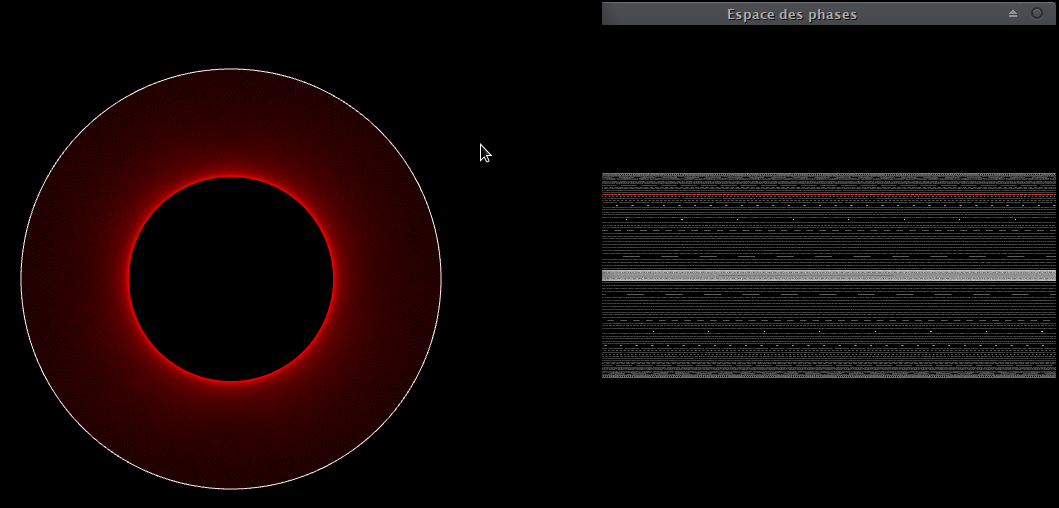
\includegraphics[width=0.8\textwidth]{TD5/trajectoires-esp-phase/traj-at-z=0.png}
\end{center}
Il s'agit évidemment d'un cas très particulier, et dès que $z\neq 0$, la symétrie par rotation est explicitement brisée. Si l'on va du côté des $z$ négatifs (billard allongé), toutes les trajectoires sont chaotiques :
\begin{center}
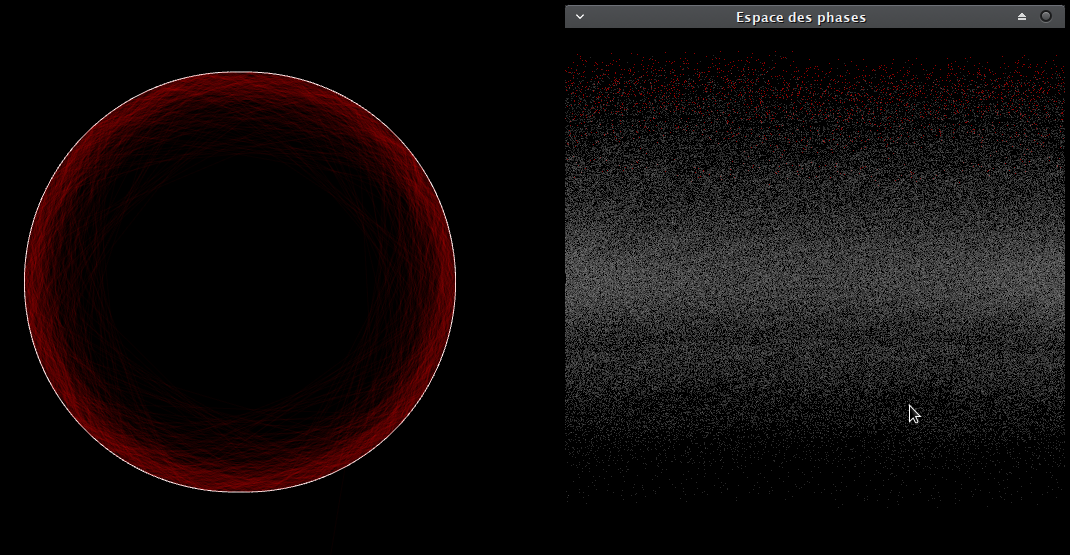
\includegraphics[width=0.8\textwidth]{TD5/trajectoires-esp-phase/traj-chaotique.png}
\end{center}
sans pour autant parcourir chacunes tout l'espace des phases, en particulier pour $z$ petit. Par contre, à partir d'environ $-0.05$, les trajectoires parcourent l'espace des phases uniformément, et on est dans une situation ergodique.\\
Pour $z>0$, l'espace des phases n'est pas entièrement chaotique, il existe de larges régions où l'on observe des trajectoires régulières quasi-périodiques, par exemple
\begin{center}
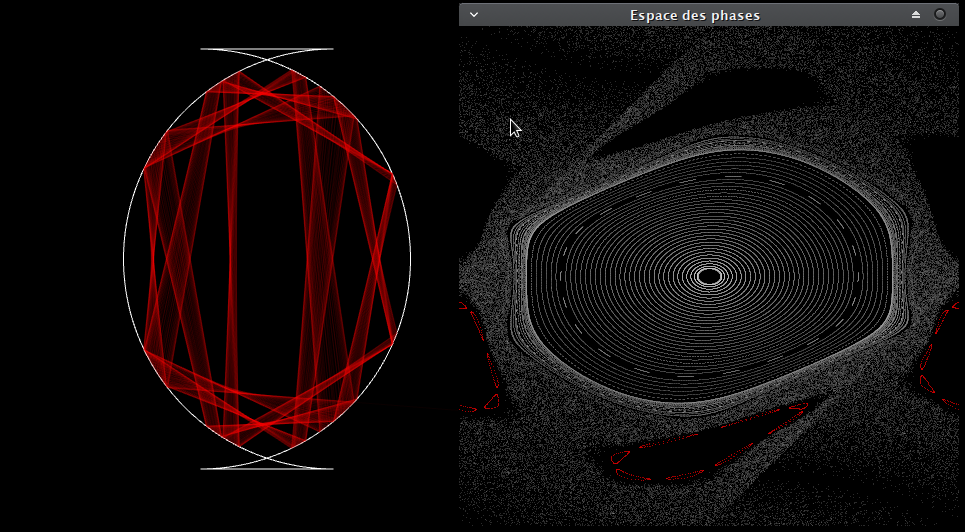
\includegraphics[width=0.8\textwidth]{TD5/trajectoires-esp-phase/traj-régulière-ordre-élevé.png}
\end{center}
ou périodiques, par exemple
\begin{center}
\includegraphics[width=0.8\textwidth]{TD5/trajectoires-esp-phase/traj-périodique.png}
\end{center}
où l'on remarque que la distribution dans l'espace des phases et en pointillée.\\
% Au dessus du "point critique" $z=+0.15$, on peut observer des trajectoires qui ne sont pas symétriques par rapport à l'axe vertical (alors que le billard l'est) :
% \begin{center}
% 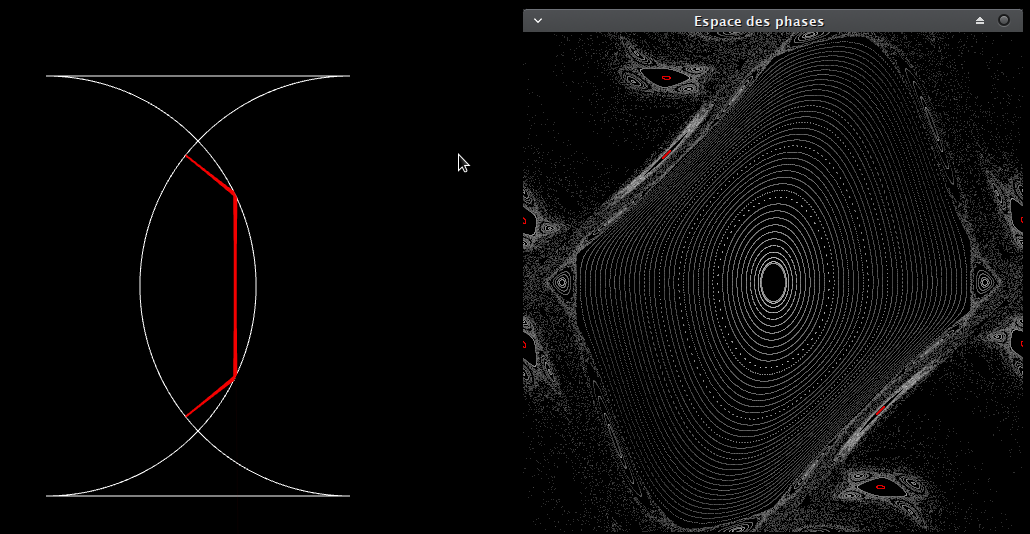
\includegraphics[width=0.8\textwidth]{TD5/trajectoires-esp-phase/traj-périodique-sym-brisée.png}
% \end{center}
% Il s'agit ici d'une trajectoire très proche d'une orbite périodique. Au point $z=+0.15$ lui-même (aux erreurs d'arrondi près), l'espace des phases est presque partout chaotique :
Il existe un "point critique" $z=+0.15$ (où le centre d'un arc de cercle tombe sur l'autre arc de cercle) où les zones régulières, présentes à droite ou à gauche de $z=+0.15$, disparaissent totalement et l'espace des phases est entièrement chaotique :
\begin{center}
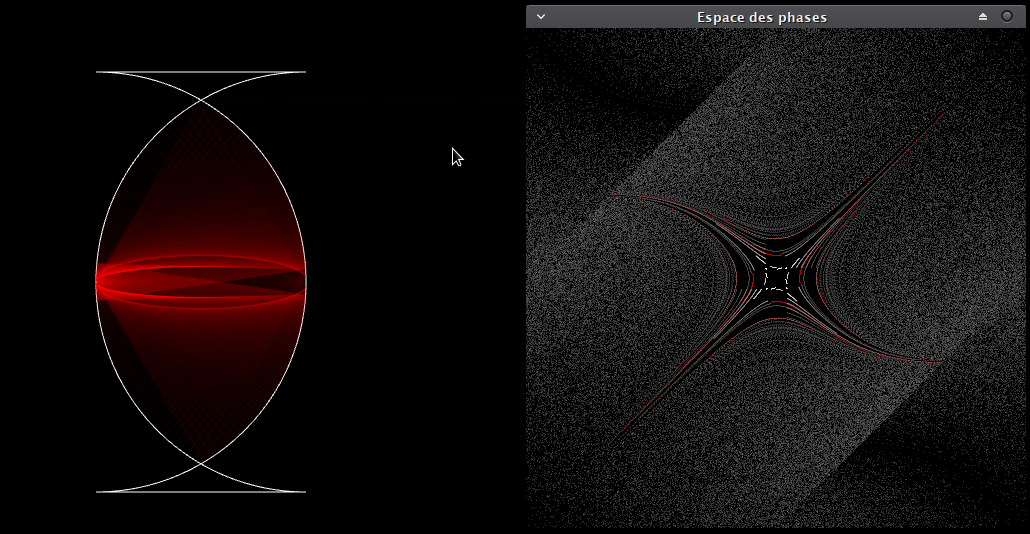
\includegraphics[width=0.8\textwidth]{TD5/trajectoires-esp-phase/traj-at-z=0.15.png}
\end{center}
Il existe de nombreux autres points où des zones régulières autre que la zone centrale apparaissent ou disparaissent.

\end{correction}

\subsection{Triangle de Reuleaux}

Un billard encore plus intéressant est composé d'arcs de cercles formant un billard avec une symétrie triangulaire. Un cas particulier est le \href{https://fr.wikipedia.org/wiki/Triangle_de_Reuleaux}{triangle de Reuleaux}, où les centres des arcs de cercle coïncident avec leur sommet opposé :
\begin{center}
  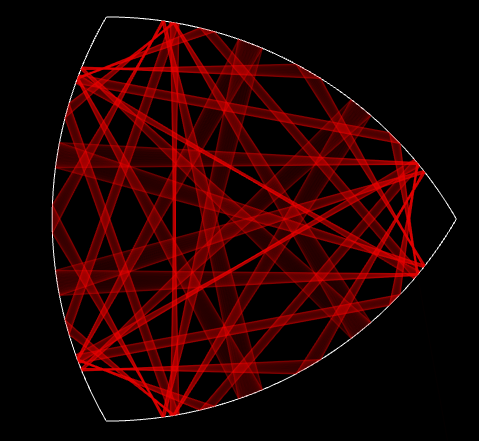
\includegraphics[height=19em]{TD5/triangle-reuleaux.png}
\end{center}

Modifiez le programme précédent (vous pourrez le dupliquer en un fichier \inline{main_sec543.cpp}) pour implémenter un tel billard. La variable $z$ pourra être utilisée pour modifier l'inverse du rayon de courbure des trois arcs de cercle.

Comme la symétrie du problème a changée, il est pertinent de transformer la coordonnée angulaire de l'espace des phases. Dans \filename{PhaseSpaceDistrib.h}, on pourra remplacer le calcul de \inline{i} par :
\begin{minted}{c++}
int i = lroundf( (p/M_PI+1)/2*3 * Npts ) % Npts;
\end{minted}

Notez les deux valeurs de $z$ (outre le cercle $z=3$ et le triangle $z=0$) pour lesquelles la dynamique semble partout intégrable. Notez la valeur de $z$ pour laquelle la dynamique est entièrement chaotique.

\end{document}
